%
% File acl2018.tex
%
%% Based on the style files for ACL-2017, with some changes, which were, in turn,
%% Based on the style files for ACL-2015, with some improvements
%%  taken from the NAACL-2016 style
%% Based on the style files for ACL-2014, which were, in turn,
%% based on ACL-2013, ACL-2012, ACL-2011, ACL-2010, ACL-IJCNLP-2009,
%% EACL-2009, IJCNLP-2008...
%% Based on the style files for EACL 2006 by 
%%e.agirre@ehu.es or Sergi.Balari@uab.es
%% and that of ACL 08 by Joakim Nivre and Noah Smith

\documentclass[11pt,a4paper]{article}
\usepackage[hyperref]{acl2018}
\usepackage{times}
\usepackage{latexsym}

\usepackage{url}

\usepackage{xcolor}
\newcommand{\todo}[1]{\textcolor{red}{TODO: #1}\PackageWarning{TODO:}{#1!}}
\newcommand{\red}[1]{\textcolor{red}{#1}}
\newcommand{\blue}[1]{\textcolor{blue}{#1}}
\newcommand{\yellow}[1]{\textcolor{yellow}{#1}}
\newcommand{\green}[1]{\textcolor{green}{#1}}
\newcommand{\cyan}[1]{\textcolor{cyan}{#1}}
\newcommand{\brown}[1]{\textcolor{brown}{#1}}
\newcommand{\purple}[1]{\textcolor{purple}{#1}}
\newcommand{\orange}[1]{\textcolor{orange}{#1}}

\usepackage{xspace}
\newcommand{\RE}{\texttt{RE}\xspace}
\newcommand{\NN}{\texttt{NN}\xspace}
\newcommand{\NLU}{\texttt{NLU}\xspace}
\newcommand{\NLP}{\texttt{NLP}\xspace}


%\aclfinalcopy % Uncomment this line for the final submission
%\def\aclpaperid{***} %  Enter the acl Paper ID here

%\setlength\titlebox{5cm}
% You can expand the titlebox if you need extra space
% to show all the authors. Please do not make the titlebox
% smaller than 5cm (the original size); we will check this
% in the camera-ready version and ask you to change it back.

\newcommand\BibTeX{B{\sc ib}\TeX}

\title{Combining Regular Expression Patterns with Neural Network for Natural Language Understanding}

\author{First Author \\
  Affiliation / Address line 1 \\
  Affiliation / Address line 2 \\
  Affiliation / Address line 3 \\
  {\tt email@domain} \\\And
  Second Author \\
  Affiliation / Address line 1 \\
  Affiliation / Address line 2 \\
  Affiliation / Address line 3 \\
  {\tt email@domain} \\}

\date{}

\begin{document}
\maketitle

\begin{abstract}
TBD

\end{abstract} 
\section{Introduction}

% Neural networks (\NN) have been proven to be effective in various natural language processing (\NLP) tasks, including text classification \cite{kim2014convolutional}, question answering \cite{yih2015semantic}, machine translation \cite{bahdanau2014neural}, and etc.

% However, the data-driven nature of \NN makes it heavily rely on large amount of labeled data, which is expensive and hard to produce.
% For example, when developing a dialogue system for a new domain where there is no relevant data, we can only come up with several queries based on our experience before we have user logs, which is not enough for \NN to work well.

Regular expression (\RE) is a commonly used technique to deal with natural language processing (\NLP) problems, including sentence
classification, sequence labeling, and etc~\cite{chang2014tokensregex}. For example, in dialogue system, an \RE pattern \texttt{/\textasciicircum flights? from/} can
help recognizing the sentence in Table~\ref{atis_sample} as expressing intent \emph{flights}, which indicates that the user is looking for
flight-related information. As a technique based on human-generated rules, it is explainable, tunable, and does not rely on training data,
making it widely used in industry and especially in scenarios where the training data is limited (few-shot learning)~\cite{gc2015big}.

On the other hand, since all the synonyms and variations need to be explicitly specified, the generalization ability of \RE is rather poor,
which leads to low coverage of the patterns. Therefore, in practice, \RE is often combined with data-driven methods like neural network
(\NN), where \RE is considered as an easy-to-tune method to deal with a certain fraction of cases with high-precision.

However, the value of \RE is more than that. When writing an \texttt{RE}, people actually encode their knowledge about the problem in the
pattern, which can be used to improve our data-driven models like \NN. For example, an \RE actually indicates the informative words
(\textbf{\emph{clue words}}) for its prediction.

Since \NN proves to perform generally well than other data-driven methods~\cite{kim2014convolutional, bahdanau2014neural}, in this paper,
we investigate the methods of using \RE to improve \NN. By doing this, different from the scenario where we only use high-precision
\texttt{RE}s to handle a fraction of cases, we can further make use of low-precision \texttt{RE}s, since \NN is known to be good at
tolerenting noises~\cite{xie2016disturblabel}. This also reduces the difficulty of writing \texttt{RE}s, since high-precision \texttt{RE}s
are hard to generate, and are usually more complex than low-precision ones.

% On the other side, since \NN models rely on distributed representation, they can generalize the \RE pattern so that phrases with similar meaning can also been matched, which may possibly result in better performance than using the \RE alone.

% On the other hand, instead of encoding knowledge into massive labeled data, human tend to express their knowledge in a more compact way, i.e., the rules. The rules accumulated by domain experts makes it an excellent source to compensate the shortage of labeled data.


Specifically, we explore fusing \RE with \NN in three different aspects: (1) On the \NN input side, we can use the \RE output as features
to \NN. This shares similar spirit with the stacking technique~\cite{wolpert1992stacked} and has also been used by~\cite{wangcombining17}
to incorporate knowledge base rules in short text classification.
(2) On the \NN module side, since \texttt{RE}s highlight clue words for a
specific tag, we can use \RE to guide the attention module in \NN. (3) On the \NN output side, we can combine the output of \RE and \NN in
a learnable way, so that the final output contains information from both \NN and \RE. Hu et al.~\shortcite{hu2016harnessing} also explored
this aspect by using first-order-logic (\FOL) constraints to affect the \NN output in a teacher-student network manner. Different from
their general framework, since \RE output is usually related to the label that we are trying to predict, we use a more direct way for
combination.
% However, since it is a general framework, it sacrifices some directness of the combination for its generality。
% but they are more focused on constraints that should not be broke rather than the positive signals produced by \RE.

We experiment our methods in the natural language understanding (\NLU) scenario.
We choose this task because it contains intent detection and slot filling as two subtasks, which correspond to two of the most important tasks in \NLP: sentence classification, sequence labeling. Further, this is also a task where \texttt{RE}s are heavily used in industry.

We explore both the few-shot learning setting where the data is limited and the setting with the full dataset, to see how \RE helps when we have different amounts of data.
To guide \RE annotation, we also conduct analysis on the impact of \RE complexity to the performance \NN.

Our contributions are: (1) To our knowledge, we are the first to systematically investigate methods for combining \RE and \NN. (2) The extensive experiments show that our methods clearly improve the \NN performance in both few-shot learning settings, and the settings with full dataset. (3) Our analysis provides meaningful guidance to fusing method selection, and \RE annotation as well.

\section{Problem Definition}
Describe the two major tasks: intent detection (sentence classification), slot filling (sequence labelling)
\begin{figure*}[!t]
\centering
\subfigure[Intent Detection] {
    \label{fig_overview_intent}
    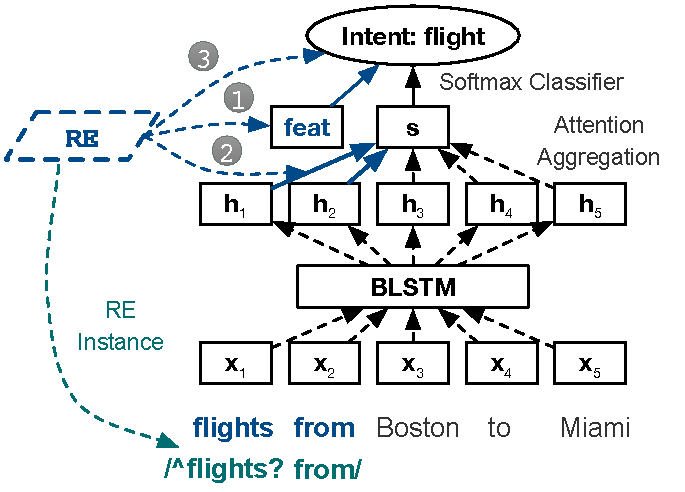
\includegraphics[width=0.8\columnwidth]{figure/re_nn_overview_intent.pdf}
}
\hspace{.5in}
\subfigure[Slot Filling (predicting slot label for \textsl{\underline{Boston}})] {
    \label{fig_overview_slot}
    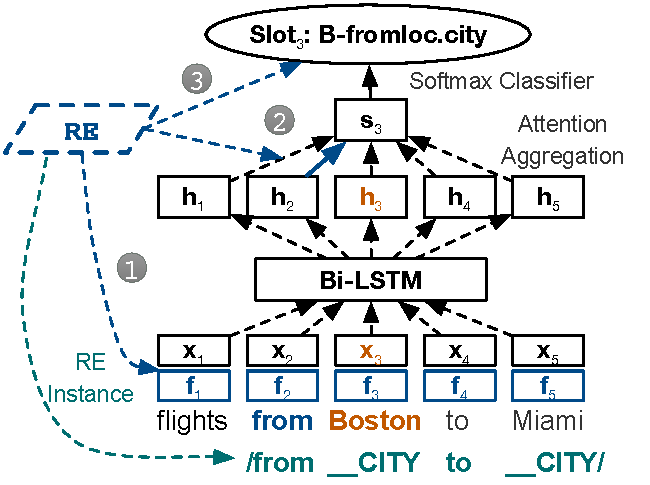
\includegraphics[width=0.8\columnwidth]{figure/re_nn_overview_slot.pdf}
}
\vspace{-3mm}
\caption{Overview of our methods. \circled{1}, \circled{2}, \circled{3} refers to the methods in
Sec.~\ref{fusion_with_input}, \ref{interact_with_module}, \ref{fusion_with_output} respectively.}
 % and the \RE that applies to the input
% sentence is shown in the bottom.}
\label{fig_overview}
\vspace{-5mm}
\end{figure*}

\section{Our Approach}
As depicted in Fig.~\ref{fig_overview}, we propose  to combine \NNs and \REs from three different angles.
 % for intent detection and slot filling.
% We present each method in the following sub-sections, starting by describing the base \NN model used by all the three methods.

\subsection{Base Models}
\label{sec:baseline} We use the Bi-directional LSTM (\BLSTM) as our base \NN model because it is effective in both intent detection and
slot filling~\cite{liu2016attention}.
% Further, to obtain sentence embedding for intent detection, we use a self-attention layer upon the \BLSTM output.

\cparagraph{Intent Detection} As shown in Fig.~\ref{fig_overview}, the \BLSTM takes as input the word embeddings $[\textbf{x}_1, ...,
\textbf{x}_n]$ of a n-word sentence, and produces a vector $\textbf{h}_i$ for each word $i$. A self-attention layer then takes in the
vectors produced by the \BLSTM to compute the sentence embedding $\textbf{s}$:
\begin{equation}
\textbf{s} = \sum_{i}{\alpha_i\textbf{h}_i}, \quad \alpha_i=\frac{\exp(\textbf{h}_i^\intercal \textbf{Wc})}{\sum_{i}{\exp(\textbf{h}_i^\intercal \textbf{Wc})}}
\label{eq:simple_att}
\end{equation}
where  $\alpha_i$ is the attention for word $i$, $\textbf{c}$ is a randomly initialized trainable vector used to select informative words for classification, and $\textbf{W}$ is a weight matrix.
Finally, $\textbf{s}$ is fed to a softmax classifier for intent classification.

\cparagraph{Slot Filling} The model for slot filling is  straightforward -- the slot label prediction is generated by a softmax classier
which takes in the \BLSTM's output $\textbf{h}_i$ and produces the slot label of word $i$. Note that attention aggregation in
Fig.~\ref{fig_overview} is only employed by the network module level method presented in Sec.~\ref{interact_with_module}.


\subsection{Using REs at the Input Level}
\label{fusion_with_input}
% Similar to the stacking technique \cite{wolpert1992stacked}, a straightforward way to combine \RE and \NN is to use the output of \RE patterns as feature, and feed them as input of \NN models.
At the input level, we use the evaluation outcomes of \REs as features which are fed to \NN models.

\cparagraph{Intent Detection}
Our \REtag for intent detection is the same as our target intent label.
% \footnote{If no \RE matches, we will assign a special tag indicating no matches. This process is applied to all the settings.}
Because real-world \REs are unlikely to be perfect, one sentence may be matched by more than one \RE. This may result in several \REtags
that are conflict with each other. For instance, the sentence \textsl{\underline{list the Delta airlines flights to Miami}} can match a
\RE: {\small \texttt{/list(\;the)?\;\_\_AIRLINE/}} that outputs tag \emph{airline}, and another \RE: {\small \texttt{/list(\,\textbackslash
w+)\{0,3\} flights?/}} that outputs tag \emph{flight}.
% \footnote{\texttt{\_\_WORD} matches a single word, which can be \texttt{/\textbackslash w+/}.}

To resolve the conflicting situations illustrated above, we average the randomly initialized trainable tag embeddings to form an aggregated
embedding as the \NN input. There are two ways to use the aggregated embedding. We can  append the aggregated embedding to either the
embedding of every input word, or the input of the softmax classifier (see \circled{1} in Fig.~\ref{fig_overview_intent}). To determine
which strategy works best, we perform a pilot study. We found that the first method causes the tag embedding to be copied many times;
consequently, the \NN tends to heavily rely on the \REtags, and the resulting performance is similar to the one given by using \REs alone
in few-shot settings. Thus, we adopt the second approach.
% In our pilot experiments on the
%first method, the tag embedding is copied so many times that tends to make the \NN heavily relies on the \REtags, making the performance
%similar to using \RE alone in few-shot settings. We therefore adopt the second method in this paper.

\cparagraph{Slot Filling} Since the evaluation outcomes of slot \REs are word-level tags,
we can simply embed and average the \REtags into a vector $\textbf{f}_i$ for each word, and append it
to the corresponding word embedding $\textbf{w}_i$ (as shown in \circled{1} in Fig.~\ref{fig_overview_slot}).
%Further, since our slot labels follow the \BIO annotation paradigm,
Note that we also extend the slot \REtags into the \BIO format, e.g., the \REtags of phrase \textsl{\underline{New York}} are \emph{B-city} and \emph{I-city} if its original tag is \emph{city}.

\subsection{Using REs at the Network Module Level}
\label{interact_with_module} At the network module level, we explore ways to utilize the clue words in the surface form of a \RE (bold blue arrows and
words in \circled{2} of Fig.~\ref{fig_overview}) to guide the attention module in \NNs.

%Since the \RE itself has already highlighted the clue words (bold blue arrows and words in \circled{2} of Fig.~\ref{fig_overview}) for its output tag, it can therefore help us guide the attention module in \NN.

\cparagraph{Intent Detection} Taking the sentence in Fig.~\ref{atis_sample} for example, the \RE: {\small\texttt{/\textasciicircum
flights?\:from/} } that leads to intent \emph{flight} means that \textsl{\underline{flights from}} are the key words to decide the intent
\emph{flight}. Therefore, the attention module in \NNs should leverage these two words to get the correct prediction. To this end, we
extend the base intent model by making two changes to incorporate the guidance from \REs.

First, since each intent has its own clue words, using a single sentence embedding for all intent labels %which is produced by only one set of attention,
would make the attention less focused.
% Considering we also know the intent that each \RE points to,
Therefore, we let each intent label $k$ use different attention $\textbf{a}_k$, which is then used to generate the sentence embedding
$\textbf{s}_k$ for that intent:
\begin{equation}
\textbf{s}_k = \sum_{i}{\alpha_{ki}\textbf{h}_i}, \quad
\alpha_{ki}=\frac{\exp(\textbf{h}_i^\intercal \textbf{W}_a\textbf{c}_k)}{\sum_{i}{\exp(\textbf{h}_i^\intercal \textbf{W}_a\textbf{c}_k)}}
\label{label_att_eq}
\end{equation}
where $\textbf{c}_k$ is a trainable vector for intent $k$ which is used to compute attention $\textbf{a}_k$, $\textbf{h}_i$ is the \BLSTM output for word $i$, and $\textbf{W}_a$ is a weight matrix.

The probability $p_k$ that the input sentence expresses intent $k$ is computed by:
\begin{equation}
p_k = \frac{\exp(logit_k)}{\sum_{k}{\exp(logit_k)}}, \quad\quad logit_k=\textbf{w}_k\textbf{s}_k + b_k
\label{label_prob_eq}
\end{equation}
where $\textbf{w}_k$, $logit_k$, $b_k$ are weight vector, logit, and bias for intent $k$, respectively.

Second, apart from indicating a sentence for intent $k$ (\textbf{\emph{positive \REs}}),
a \RE can also indicate that a sentence does not express intent $k$ (\textbf{\emph{negative \REs}}).
%Therefore, to make use of negative \REs,
We thus use a new set of attention (\textbf{\emph{negative attentions}}, in contrast to \textbf{\emph{positive attentions}}), to compute
another set of logits for each intent with Eqs.~\ref{label_att_eq} and \ref{label_prob_eq}. We denote the logits computed by positive
attentions as $logit_{pk}$, and those by negative attentions as $logit_{nk}$, the final logit for intent $k$ can then be calculated as:
\begin{equation}
logit_k = logit_{pk} - logit_{nk}
\end{equation}

To use \REs to guide attention, we add an attention loss to the final loss:
\begin{equation}
%loss_{att} = \sum_{k}{m_k\sum_{i}{t_{ki}\log(\alpha_{ki})}}
loss_{att} = \sum_{k}{\sum_{i}{t_{ki}\log(\alpha_{ki})}}
\label{att_loss}
\end{equation}
where $t_{ki}$ is set to $0$ when none of the matched \REs (that leads to intent $k$) marks word $i$ as a clue word -- otherwise $t_{ki}$
is set to $1/l_{k}$, where $l_k$ is the number of clue words
% mark by \RE
for intent $k$ (if no matched \RE leads to intent $k$, then $t_{k*}=0$).
%$m_k$ is a 0-1 indicator that is set to 1 when there is a matched \RE that leads to intent $k$.
We use Eq.~\ref{att_loss}
to compute the positive attention loss, $loss_{att\_p}$, for positive \REs and negative attention loss, $loss_{att\_n}$, for negative ones.
The final loss is computed as:
\begin{equation}
loss = loss_{c} + \beta_p loss_{att\_p} + \beta_n loss_{att\_n}
\end{equation}
where $loss_{c}$ is the original classification loss, $\beta_p$ and $\beta_n$ are weights for the two attention losses.

\cparagraph{Slot Filling}
%While we can apply the same \textbf{\emph{two-side attention}} (positive and negative attention) mechanism
%as we do in intent prediction, we will face an efficiency problem in slot filling.
The \textbf{\emph{two-side attention}} (positive and negative attention) mechanism introduced for intent prediction is unsuitable for slot
filling. Because for slot filling, we need to compute attention for each word, which demands more computational and memory resources than
doing that for intent detection\footnote{Since we need to assign a label to each word, if we still compute attention for each slot label,
we will have to compute $2\times L \times n^2$ attention values for one sentence. Here, $L$ is the number of tags and $n$ is the sentence
length. The \BIO tagging format will further double the number of tags.}.

Because of the aforementioned reason, we use a simplified version of the two-side attention, where all the slot labels share the same set
of positive and negative attention. Specifically, to predict the slot label of word $i$, we use the following equations, which are similar
to Eq.~\ref{eq:simple_att}, to generate a sentence embedding $\textbf{s}_{pi}$ with regard to word $i$ from positive attention:
\begin{equation}
\textbf{s}_{pi} = \sum_{j}{\alpha_{pij}\textbf{h}_j}, \quad \alpha_{pij}=\frac{exp(\textbf{h}_j^T\textbf{W}_{sp}\textbf{h}_i)}{\sum_{j}{exp(\textbf{h}_j^T\textbf{W}_{sp}\textbf{h}_i)}}
\label{eq:slu_simple_att}
\end{equation}
where $\textbf{h}_i$ and $\textbf{h}_j$ are the \BLSTM outputs for word $i$ and $j$ respectively, $\textbf{W}_{sp}$ is a weight matrix, and
$\alpha_{pij}$ is the positive attention value for word $j$ with respect to word $i$. Further, by replacing $\textbf{W}_{sp}$ with
$\textbf{W}_{sn}$, we use  Eq.~\ref{eq:slu_simple_att} again to compute negative attention and generate the corresponding sentence
embedding $\textbf{s}_{ni}$.

Finally, the prediction $\textbf{p}_i$ for word $i$ can be calculated as:
\begin{equation}
\begin{split}
\textbf{p}_i = \softmax((\textbf{W}_p [\textbf{s}_{pi}; \textbf{h}_i] + \textbf{b}_p) \\- (\textbf{W}_n [\textbf{s}_{ni}; \textbf{h}_i] + \textbf{b}_n))
\end{split}
\end{equation}
where $\textbf{W}_{p}$, $\textbf{W}_{n}$, $\textbf{b}_{p}$, $\textbf{b}_{n}$ are weight matrices and bias vectors for positive and negative attention, respectively. Here we append the \BLSTM output $\textbf{h}_i$ to $\textbf{s}_{pi}$ and $\textbf{s}_{ni}$ because the word $i$ itself also plays a crucial part in identifying its slot label.

\subsection{Using REs at the Output Level}
\label{fusion_with_output} At the output level, \REs are used to amend the output of \NNs. At this level, we take the same approach used
for intent detection and slot filling (see \circled{3} in Fig.~\ref{fig_overview}).

% Therefore, instead using a teach-student framework, this enables us to directly influence the logits of each label in a trainable way, so that we do not need to assign a weight for each pattern, and significantly reduces the number of hyper-parameters.

As mentioned in Sec.~\ref{re_desc}, the slot \REs used in the output level only produce a simplified version of target slot labels, for which
we can further
%Since the \REtag is related to the slot label, we can further
annotate their corresponding target slot labels.
% To make connections between the \RE tag and the slot label, we further annotate all the slot labels that the output tag may lead to.
For instance, a \RE that outputs \emph{city} can lead to three slot labels: \emph{fromloc.city}, \emph{toloc.city},
\emph{stoploc.city}.
% Actually, annotating this kind of connections is not difficult, since the \RE tags are generally somewhat related to the target label that we are trying to predict, otherwise the \RE tags will not be able to provide useful information for the prediction.

Let $z_k$ be a 0-1 indicator of whether there is at least one matched \RE that leads to target label $k$ (intent or slot label), the final
logits of label $k$ for a sentence (or a specific word for slot filling) is:
\begin{equation}
logit_k = logit'_k + w_k z_k
\end{equation}
where $logit'_k$ is the logit produced by the original \NN, and $w_k$ is a trainable weight indicating the overall confidence for \REs that
lead to target label $k$. Here we do not assign a trainable weight for each \RE because it is often that only a few sentences match a \RE.

We modify the logit instead of the final probability because a logit is an unconstrained real value, which matches the property of $w_k
z_k$ better than probability. Actually, when performing model ensemble,
% kagglers have also proved emperically that,
ensembling with logits is often empirically better than with the final probability\footnote{ An example can be found in the ensemble
version that Juan et al.~\shortcite{juan2016field} used in the Avazu Kaggle competition. }. This is also the reason why we choose to
operate on logits in Sec.~\ref{interact_with_module}.

\section{Evaluation Methodology}
Our experiments aim to answer two main questions: (1) Does \RE patterns helps? (2) Which combination method works, and when does it work? (3) Does the size of training data influence the improvements? (4) Is our combination method compatible to other more sophisticated \NN architectures?  

\subsection{Datasets}
ATIS (Airline Travel Information Systems) dataset \cite{hemphill1990atis} is a widely used benchmark in \NLU research. It contains audio recordings of people making flight reservations, which involves queries like asking flights, airlines, meal, abbreviations and etc. We follow the setup used by \cite{liu2016attention}, with 4978 queries for training and 893 for test. There are 127 distinct slot labels and 18 different intents. Besides, numbers are also replaced with special tokens like \emph{DIGIT*m}, where m is the number of digits in the original string.

To answer question (3), we also explore a few shot learning setting. Specifically, for intent detection, we randomly select 5, 10, 20 instances from the training set for each intent to form the few-shot learning training set. As for slot filling, since one sentence typically involves multiple slot labels, we can only make the number of training instances for each label as close to the target number as possible. Therefore, we further explore settings with 1, 3, 5, 10, 20 shots. Specifically, we first sort the slot labels by frequence, and randomly select sentence for the least-frequence label first. After that, we move to the adjacent label which is slightly more frequent, and make sure the number of training instances meet the threshold. $k_1$-shot dataset is contained by $k_2$-shot dataset if $k_1 < k_2$, so that the \RE patterns can be reused through different settings. We use the original test set for both intent detection and slot filling.

Since most few-shot learning methods require either extra classes or classes with enough data for training, we also explore a new setting for intent detection to make fair comparison with existing few-shot learning methods. Specifically, we make the 3 most frequent intents to have 300 training instances, and the rest of the few-shot learning dataset remains untouched, so that we can ensure enough training data to make existing few-shot learning methods to work.

The \RE patterns are annotated only based on the few-shot learning datasets, but word lists like city lists are collected using the full dataset. Typically, annotating intent patterns are simple, which takes about 1 minutes to yield one pattern, and we collected 54 patterns in total, and the three combination methods share the same set of patterns. Similarly, annotating slot filling patterns to provide feature or modify output is also easy since it does not require high-precision. It also takes about 1 minutes to yield one pattern, and there are 60 patterns. However, annotating slot filling patterns to guide attention is difficult, since the clue words need careful determination. Tiypically, we need about 2-5 minutes to generate one pattern, and we obtained 115 patterns. These patterns a generated in a single run, and not modified during experiments.


\subsection{Experimental Setup}
\paragraph{Hyper-parameters}
We use similar hyper-parameters to \cite{liu2016attention} and achieves comparative results in the original dataset. Specifically, we have batch size 16, dropout probability 0.5, Bi-LSTM size 200 (100 for each direction), attention loss weight 16 (both positive and negative) for few-shot, and weight 1 when we have more data (see Section \ref{sec:experiments} for details). We use 100-dimensional GloVe \cite{pennington2014glove} word vector trained on Wikipedia and Gigaword, and Adam optimizer \cite{kingma2014adam} with learning rate 0.001.

\paragraph{Evaluation Metric}
Intent: accuracy, macro P, R, F1

Slot: micro/macro P, R, F1

\paragraph{Naming Conventions}
\texttt{raw} refers to attentional Bi-LSTM for intent detection and vanila Bi-LSTM for slot filling, \texttt{two} refers to Bi-LSTM with positive-negative attention (but without attention guidance), \texttt{+feat} means add \RE output as feature, \texttt{+posi} and \texttt{+neg} refers to use positive and negative attention loss respectively, \texttt{+both} refers to use both positive and negative attention, \texttt{RE} refers to using the \RE pattern output as prediction directly, \texttt{mem} means adding the memory module \cite{kaiser2017learning} to \texttt{raw}, \texttt{joint} means the joint model \cite{liu2016attention} which achives state-of-art result in ATIS dataset. 





\section{Experimental Results}
\label{sec:experiments}

\subsection{Full Few-Shot Learning}
To answer \textbf{Q1} , we first explore the full few-shot learning scenario.

\begin{table*}
\setlength{\tabcolsep}{0.23em}
\centering
\small{
\begin{tabular}{|l|l|c|c|c|c|c|c|}

\hline
\multirow{3}{*}{\textbf{Model Type}} & \multirow{3}{*}{\textbf{Model Name}}  & \multicolumn{3}{|c|}{\textbf{Intent}} & \multicolumn{3}{|c|}{\textbf{Slot}} \\
\cline{3-8}
&  & \multicolumn{1}{|c|}{\textbf{5-shot}} & \multicolumn{1}{|c|}{\textbf{10-shot}} & \multicolumn{1}{|c|}{\textbf{20-shot}}
& \multicolumn{1}{|c|}{\textbf{5-shot}} & \multicolumn{1}{|c|}{\textbf{10-shot}} & \multicolumn{1}{|c|}{\textbf{20-shot}}  \\
\cline{3-8}
&  & \multicolumn{3}{|c|}{\textbf{Macro-F1 / Accuracy}} & \multicolumn{3}{|c|}{\textbf{Macro-F1 / Accuracy}} \\
\hline

\rowcolor{Gray}Base Model & \BLSTM & 45.28 / 60.02 & 60.62 / 64.61 & 63.60 / 80.52
& 60.78 / 83.91 & 74.28  / 90.19 & 80.57 / 93.08  \\
\hline Input Level & \texttt{+feat} & 49.40 / 63.72 & 64.34 / 73.46 & 65.16 / 83.20
& \textbf{66.84} / \textbf{88.96} & 79.67 / \textbf{93.64} & 84.95 / 95.00  \\
\hline

\rowcolor{Gray}  & \texttt{+logit} & 46.01 / 58.68 & 63.51 / 77.83 & 69.22 / \textbf{89.25}
& 63.68 / 86.18 & 76.12 / 91.64  & 83.71 / 94.43 \\
\cline{2-8}

\rowcolor{Gray} \multirow{-2}{*}{Output Level}& \texttt{+hu16} & 47.22 / 56.22 & 61.83 / 68.42 & 67.40 / 84.10
& 63.37 / 85.37 & 75.67 / 91.06 & 80.85 / 93.47  \\
\hline \multirow{2}{*}{\vspace{-2.2em}\tabincell{c}{Network Module \\ Level}} & \texttt{+two} & 40.44 / 57.22 & 60.72 / 75.14 & 62.88 /
83.65
& 60.38 / 83.63 & 73.22 / 90.08 & 79.58 / 92.57  \\
\cline{2-8} & \texttt{+two+posi} & 50.90 / 74.47 & 68.69 / 84.66 & 72.43 / 85.78
& 59.59 / 83.47 & 73.62 / 89.28 & 78.94 / 92.21 \\
\cline{2-8} & \texttt{+two+neg} & 49.01 / 68.31 & 64.67 / 79.17 & 72.32 / 86.34
& 59.51 / 83.23 & 72.92 / 89.11 & 78.83 / 92.07 \\
\cline{2-8} & \texttt{+two+both} & \textbf{54.86} / \textbf{75.36} & \textbf{71.23} / \textbf{85.44} & \textbf{75.58} / 88.80
& 59.47 / 83.35 & 73.55 / 89.54 & 79.02 / 92.22 \\
\hline
\rowcolor{Gray} & \texttt{+mem} & - & - & - & 61.25 / 83.45 & 77.83 / 90.57 & 82.98 / 93.49 \\
\cline{2-8}
\rowcolor{Gray} \multirow{-2}{*}{Few-Shot Model}  & \texttt{+mem+feat} & - & - & - & 65.08 / 88.07 & \textbf{80.64} / 93.47 & \textbf{85.45} / \textbf{95.39} \\
\hline
\hline
RE Output & \REO & \multicolumn{3}{|c|}{70.31 / 68.98} & \multicolumn{3}{|c|}{42.33 / 70.79} \\
\hline
\end{tabular}
} \caption{Results on Full Few-Shot Learning Settings. For slot filling, we do not distinguish full and partial few-shot learning settings
(see Sec.~\ref{sec_datasest}).}
% \caption{\cyan{Results on full few-shot learning settings (slot filling does not distinguish full/partial few-shot).}}
% \caption{\cyan{Results on Full Few-Shot Learning. Note that, since frequent slot labels exceed the target shot count, for slot filling, we use the same dataset for both full and partial few-shot settings.}}
% \caption{\cyan{Results on Full Few-Shot Learning. We use the same dataset for both full and partial few-shot learning.}}
\label{tab_full_few}
\vspace{-1em}
\end{table*}

\cparagraph{Intent Detection} As shown in Table \ref{tab_full_few}, except for 5-shot, all approaches improve the baseline \texttt{BLSTM}.
Our network-module-level methods give the best performance because our attention module directly receives signals from the clue words in
\REs that contain more meaningful information than the \REtag itself used by other methods. We also observe that since negative \REs are
derived from positive \REs with some noises, \texttt{posi} performs better than \texttt{neg} when the amount of available data is limited.
However, \texttt{neg} is slightly better in 20-shot, possibly because negative \REs significantly outnumbers the positive ones. Besides,
\tatt alone works better than the \texttt{BLSTM} when there are sufficient data, confirming the advantage of our two-side attention
architecture.

As for other proposed methods, the output level method (\texttt{logit}) works generally better than the input level method (\texttt{feat}),
except for the 5-shot case. We believe this is due to the fewer number of \RE related parameters and the shorter distance that the gradient
needs to travel from the loss to these parameters -- both make \texttt{logit} easier to train. However, since \texttt{logit} directly
modifies the output, the final prediction is more sensitive to the insufficiently trained weights in \texttt{logit}, leading to the
inferior results in the 5-shot setting.

To compare with existing methods of combining \NN and rules, we also implement the teacher-student network~\cite{hu2016harnessing}. This
method lets the \NN learn from the posterior label distribution produced by \FOL rules in a teacher-student framework, but requires
considerable amounts of data. Therefore, although both \texttt{hu16} and \texttt{logit} operate at the output level, \texttt{logit} still
performs better than \texttt{hu16} in these few-shot settings, since \texttt{logit} is easier to train.
% \todo{try to acknowledge that \texttt{hu16} belongs to \emph{fusion in output}}

% We can also see that, the improvements from \RE decreases as we have more data,
% which is reasonable since as we have more data, the information contained in the data will have more overlap with the information in \RE.

It can also be seen that starting from 10-shot, \texttt{two+both} significantly outperforms pure \REO. This suggests that by using our
attention loss to connect the distributional representation of the \NN and the clue words of \REs, we can generalize \RE patterns within a
\NN architecture by using a small amount of annotated data.


\cparagraph{Slot Filling}
Different from intent detection, as shown in Table \ref{tab_full_few}, our attention loss does not work for slot filling.
% \footnote{Negative pattern works even worse, we therefore only show the results of positive pattern here}.
The reason is that the slot label of a \textbf{\emph{target word}} (the word for which we are trying to predict a slot label) is decided
mainly by the semantic meaning of the word itself, together with 0-3 phrases in the context to provide supplementary information. However,
our attention mechanism can only help in recognizing clue words in the context, which is less important than the word itself and have
already been captured by the \BLSTM, to some extent. Therefore, the attention loss and the attention related parameters are more of a
burden than a benefit. As is shown in Fig.~\ref{atis_sample}, the model recognizes \textsl{\underline{Boston}} as \emph{fromloc.city}
mainly because \textsl{\underline{Boston}} itself is a city, and its  context word \textsl{\underline{from}} may have already been captured
by the \BLSTM and our attention mechanism does not help much. By examining the attention values of \texttt{+two} trained on the full
dataset, we find that instead of marking informative context words, the attention tends to concentrate on the target word itself. This
observation further reinforces our hypothesis on the attention loss.

On the other hand, since the \REtags provide extra information, such as type, about words in the sentence, \texttt{logit} and \texttt{feat}
generally work better. However, different from intent detection, \texttt{feat} only outperforms \texttt{logit} by a margin. The is because
\texttt{feat} can use the \REtags of all words to generate better context representations through the \NN, while \texttt{logit} can only
utilize the \REtag of the target word before the final output layer. As a result, \texttt{feat} actually gathers more information from \REs
and can make better use of them than \texttt{logit}. Again, \texttt{hu16} is still outperformed by \texttt{logit}, possibly due to the
insufficient data support in this few-shot scenario. We also see that even the \texttt{BLSTM} outperforms \REO in 5-shot, indicating while
it is hard to write high-quality \RE patterns, using \REs to boost \NNs is still feasible.

% It is not surprising because this is not true 5-shot setting, extra data still exists for frequent patterns since one sentence may contain multiple slots.

%\cparagraph{In short}
\cparagraph{Summary} The amount of extra information that a \NN can utilize from the combined \REs significantly affects the resulting
performance. Thus, the attention loss methods work best for intent detection and \texttt{feat} works best for slot filling. We also see
that the improvements from \REs decreases as having more training data. This is not surprising because the implicit knowledge embedded in
the \REs are likely to have already been captured by a sufficient large annotated dataset and in this scenario using the \REs will bring in
fewer benefits.

\subsection{Partial Few-Shot Learning}
To better understand the relationship between our approach and existing few-shot learning methods, we also implement the memory network
method \cite{kaiser2017learning} which achieves good results in various few-shot datasets. We adapt their open-source code, and add their
memory module (\texttt{mem}) to our \BLSTM model.

\begin{table}
\setlength{\tabcolsep}{0.23em}
\centering
\small{
\begin{tabular}{|l|c|c|c|}

\hline
\multirow{2}{*}{\textbf{Model}}  & \multicolumn{1}{|c|}{\textbf{5-shot}} & \multicolumn{1}{|c|}{\textbf{10-shot}} & \multicolumn{1}{|c|}{\textbf{20-shot}}  \\
\cline{2-4}
 & \multicolumn{3}{|c|}{\textbf{Macro-F1 / Accuracy}}   \\
\hline
\rowcolor{Gray} \texttt{BLSTM} & 64.73 / 91.71 & 78.55 / 96.53 & 82.05 / 97.20 \\
\hline
\texttt{+hu16} & 65.22 / 91.94 & 84.49 / 96.75 & 84.80 / 97.42 \\
\hline
\rowcolor{Gray} \texttt{+two} & 65.59 / 91.04 & 77.92 / 95.52 & 81.01 / 96.86 \\
\hline
\texttt{+two+both} & 66.62 / 92.05 & 85.75 / 96.98 & \textbf{87.97} / \textbf{97.76} \\
\hline
\rowcolor{Gray} \texttt{+mem} & 67.54 / 91.83 & 82.16 / 96.75 & 84.69 / 97.42 \\
\hline
\texttt{+mem+posi} & \textbf{70.46} / \textbf{93.06} & \textbf{86.03} / \textbf{97.09} & 86.69 / 97.65 \\
\hline

\end{tabular}
} \caption{Intent Detection Results on Partial Few-Shot Learning Setting.} \label{tab_intent_few_fill} \vspace{-1em}
\end{table}

Since the memory module requires to be trained on either many few-shot classes or several classes with extra data,
we expand our full few-shot dataset for intent detection, so that the top 3 intent labels have 300 sentences (partial few-shot).

As shown in Table~\ref{tab_intent_few_fill}, \texttt{mem} works better than \BLSTM, and our attention loss can be further combined with the memory module (\texttt{mem+posi}), with even better performance. %and achieves better results.
% our attention loss also makes clear improvements in this setting.
\texttt{hu16} also works here, but  worse than \texttt{two+both}.
% Further, the attention loss can also be combined with the memory module (\texttt{mem+posi}), and achieves better results than \texttt{mem} alone.
Note that, the memory module requires the input sentence to have only one embedding, thus we only use one set of positive attention for combination.

As for slot filling, since we already have extra data for frequent tags in the original few-shot data (see Sec.~\ref{sec_datasest}), we use
them directly to run the memory module. As shown in the bottom of Table \ref{tab_full_few}, \texttt{mem} also improves the base \BLSTM, and
gains further boost when it is combined with our \texttt{feat} method\footnote{For compactness, we only combine the best method in each
task with \texttt{mem}, but others can also be combined.}.
% \footnote{
% \texttt{logit} may not be able to applied to methods with other output form, e.g., matching based method~\cite{koch2015siamese}.}.

% NOTE: since we have more data here, the importance of attention guidance is not that crucial as in the previous more strict few-shot leanring setting. Therefore, the weight of attention loss is reduced to 1 in this setting and the following full dataset setting,


\subsection{Full Dataset}

\begin{table}
\setlength{\tabcolsep}{0.23em}
\centering
\small{
\begin{tabular}{|l|c|c|}

\hline
\multirow{2}{*}{\textbf{Model}} & \textbf{Intent} & \textbf{Slot} \\
\cline{2-3}
  & \textbf{\scriptsize Macro-F1/Accuracy} &  \textbf{\scriptsize Macro-F1/Micro-F1} \\
\hline
\rowcolor{Gray} \texttt{BLSTM} & 92.50 / 98.77  & 85.01 / 95.47\\
\hline
\texttt{+feat} & 91.86 / 97.65 & 86.7 / 95.55\\
\hline
\rowcolor{Gray} \texttt{+logit} & 92.48 / 98.77 & 86.94 / 95.42  \\
\hline
\texttt{+hu16} & 93.09 / 98.77 & 85.74 / 95.33  \\
\hline
\rowcolor{Gray} \texttt{+two} & 93.64 / 98.88  & 84.45 / 95.05\\
% \hline
% two+posi & 93.02 & 98.88 \\
% \hline
% two+neg & 93.92 & \textbf{98.99} \\
\hline
\texttt{+two+both }& \textbf{96.20} / \textbf{98.99} & 85.44 / 95.27 \\
\hline
\rowcolor{Gray} \texttt{+mem} & 93.42 / 98.77 & 85.72 / 95.37\\
\hline
\texttt{+mem+posi/feat} & 94.36 / \textbf{98.99} & \textbf{87.82} / \textbf{95.90} \\
\hline
\hline
\rowcolor{Gray} L\&L16 & - / 98.43 & - / 95.98\\
\hline

\end{tabular}
}
\caption{Results on Full Dataset. The left side of `$/$' applies for intent, and the right side for slot.}
\label{tab_full}
\vspace{-1em}
\end{table}

To answer \textbf{Q2}, we also evaluate our methods on the full dataset. As seen in Table \ref{tab_full}, for intent detection, while
\texttt{two+both} still works, \texttt{feat} and \texttt{logit} no longer give improvements.
% the clue words marked by \RE still provide useful information to \NN (\texttt{two+both}),
% but the \REtag is not very useful (\texttt{feat} and \texttt{logit}).
This shows that since both \REtag and annotated data provide intent labels for the input sentence, the value of the extra noisy tag from \RE become limited as we have more annotated data.
% comparated with the knowledge learned from labeled data, the \REtag is much more noisy.
However, as there is no guidance on attention in the annotations, the clue words from \REs are still useful. Further, since \texttt{feat}
concatenates \REtags at the input level, the powerful \NN makes it more likely to overfit than \texttt{logit}, therefore \texttt{feat}
performs even worse when compared to the \BLSTM.
% This shows that, although the informative words marked by \RE still helps, the low-performance \RE output no longer works when the labeled data is sufficient. While \NN can learn to assign low weights for \RE output in \texttt{logit}, the noise coming from the input feature is hard to eliminate, and therefore leading to bad results of \texttt{feat}.

As for slot filling, \texttt{feat} and \texttt{logit} are still effective. This shows that the word type information contained in the
\REtags is still hard to be learned even when we have more annotated data.
% the output of the \RE used for \texttt{feat} and \texttt{logit} provides extra information to help \NN better understand the target word (e.g., entity type), which is hard to inferred by \NN itself.
% The reason is probably that the output of the \RE used for \texttt{feat} and \texttt{logit} is only the entity part of the slot label, which is only indirectly connected to the prediction target. The noise contained in the indirectness makes \NN relies less on the \RE output, and therefore is less sensitive to the wrong predictions made by \RE as they do in intent detection.
Moreover, different from few-shot settings, \texttt{two+both} has a better macro-F1 score than the \texttt{BLSTM} for this task, suggesting
that better attention is still useful when the base model is properly trained.

Again, \texttt{hu16} outperforms the \texttt{BLSTM} in both tasks, showing that although the \REtags are noisy, their teacher-student
network can still distill useful information. However, \texttt{hu16} is a general framework to combine \FOL rules, which is more indirect
in transferring knowledge from rules to \NN than our methods. Therefore, it is still  inferior to attention loss in intent detection and
\texttt{feat} in slot filling, which are designed to combine \REs.
% The reason that it still performs worse than attention loss intent detection and in slot filling, is

Further, \texttt{mem} generally works in this setting, and can receive further improvement
%we can also make improvements
by combining our fusion methods.
We can also see that \texttt{two+both} works clearly better than the state-of-art method (\LL) in intent detection, which jointly models the two tasks. And \texttt{mem+feat} is comparative to \LL in slot filling.
% \red{We can also see that our base model achieves comparative results to the joint model of  Liu and Lane~\shortcite{liu2016attention}, which achieves state-of-art results on the ATIS data.}
% \footnote{
% Since slot filling is evaluated in phrase level, there is almost no difference in F1 when we convert the prediction on our split data format to the original format (see Section \ref{sec_datasest})}.
% Besides, the state-of-art results on the ATIS data produced by \cite{liu2016attention} is also included (\LL). We can see that our base \BLSTM model achieves comparative results to \LL, confirming that the improvements from our fusion method does not come from the inferior ability of the base model), making our results still comparatable to \LL.}.
%\red{The analysis on different settings in the sections above together answer question (3).}

\subsection{Impact of the RE Complexity}
\label{sec_complexity}
\begin{table}
\setlength{\tabcolsep}{0.23em}
\centering
\small{
\begin{tabular}{|l|c|c|c|c|}

\hline
\multirow{3}{*}{\textbf{Model}}  & \multicolumn{2}{|c|}{\textbf{Intent}} & \multicolumn{2}{|c|}{\textbf{Slot}}  \\
\cline{2-5}
  & \multicolumn{2}{|c|}{\textbf{\scriptsize Macro-F1 / Accuracy}} & \multicolumn{2}{|c|}{\textbf{\scriptsize Macro-F1 / Micro-F1}}  \\
\cline{2-5}
  & \textbf{\scriptsize Complex} & \textbf{\scriptsize Simple} & \textbf{\scriptsize Complex} & \textbf{\scriptsize Simple} \\
\hline
\rowcolor{Gray} \texttt{BLSTM} & \multicolumn{2}{|c|}{63.60 / 80.52} & \multicolumn{2}{|c|}{80.57 / 93.08}  \\
\hline
\texttt{+feat }& 65.16/\textbf{83.20} & \textbf{66.51}/80.40 & \textbf{84.95/95.00} & 83.88/94.71 \\
\hline
\rowcolor{Gray} \texttt{+logit} & \textbf{69.22/89.25} & 65.09/83.09 & \textbf{83.71/94.43} & 83.22/93.94  \\
\hline
\texttt{+both} & \textbf{75.58/88.80} & 74.51/87.46 & - & - \\
\hline
\end{tabular}
} \caption{Results on 20-Shot Data with Simple \REs. \texttt{+both} refers to \ptatt\texttt{+both} for short.} \label{tab_simple}
\vspace{-1em}
\end{table}

%This section tries to answer
We now discuss how the \RE complexity affects the performance of the combination.
%Since enriching the phrases in a \RE group with $|$ is usually easier adding new groups,
We choose to control the \RE complexity by modifying the number of groups.
%As discussed in Sec.~\ref{re_desc}, more \RE groups will lead to better precision.
%
Specifically, we reduce the number of groups for existing \REs to decrease \RE complexity.
To mimic the process of writing simple \REs from scratch, we try our best to keep the key \RE groups.
For intent detection, all the \REs are reduced to at most 2 groups. % (groups matching a sequence of any words are excluded),
% and 17 \REs are simplified.
As for slot filling, we also reduce the \REs to at most 2 groups, and for some simples case, we further reduce them into  word-list patterns, e.g., \texttt{(\_\_CITY)}.
% In total, 21 \REs are simplified.
%\red{As for slot filling, since the \REs with more than 2 groups are limited (only 7), we choose a more aggressive strategy that all the \REs are reduced to word-list patterns, e.g., \texttt{(\_\_CITY)}.
%However, the \REs trying to tag a \RE group that matches a number or a common word can have at most 2 groups, since it is not distinguishable at all without some context.
%In total, 21 \REs are affected.}

As shown in Table \ref{tab_simple}, the simple \REs already deliver clear improvements to the base \NN models, which shows the
effectiveness of our methods, and indicates that simple \REs are quite cost-efficient since these simple \REs only contain 1-2 \RE groups
and thus very easy to produce. We can also see that using complex \REs generally leads to better results compared to using simple \REs.
This indicates that when considering using \REs to improve a \NN model, we can start with simple \REs, and gradually increase the \RE
complexity to improve the performance over time\footnote{We do not include results of \texttt{both} for slot filling since its \REs are
different from \texttt{feat} and \texttt{logit}, and we have already shown that the attention loss method does not work for slot filling.}.


%simple \REs generally lead to worse results, indicating that we should write complex \REs to get better performance if the cost is affordable.
%Further, the results of simple \REs are still better than the base \BLSTM, showing that in practice, we can safely start with simple \REs, and increase the complexity gradually

% \subsection{Key Conclusion}
% We summarize the key conclusions from the experiments above here:
% (1) The amount of extra information that \NN can learn from \RE influences the fusion performance most. Therefore, attention loss methods works best for intent detection and \texttt{feat} works best for slot filling.
% (2) The improvements from \RE decreases as we have more training data.
% (3) Our fusion methods are compatible with existing few-shot learning methods like \texttt{mem}.
% (4) Complex \RE leads to better fusion performance.
% \todo{Is this section necessary?}

\section{Related Work}

\cparagraph{NN with Rules}
% Recent efforts that try to fuse \NN and rules and be summarized in 4 aspects:
% Recent efforts on fusing \NN and rules can be summarized as follows.
On the initialization side, Li et al.~\shortcite{li2017initializing} uses important n-grams to initialize the convolution filters. 
% so that \NN can capture key n-grams in early training stage. 
On the input side, Wang et al.~\shortcite{wang2017combining} uses knowledge base rules to find relevant concepts for short texts to augment input.
On the output side,
% the teacher-student framework is widely used to let \NN learn from the posterior label distribution produced by \FOL rules~\cite{hu2016harnessing,hu2016deep,guo2017knowledge}.
Hu et al.~\shortcite{hu2016harnessing,hu2016deep} and Guo et al.~\shortcite{guo2017knowledge} use \FOL rules to rectify the output probability of \NN, and then let \NN learn from the rectified distribution in a teacher-student framework.
% \cite{guo2017knowledge} followed the same framework and adapted it to the knowledge graph embedding task.
Xiao et al.~\shortcite{xiao2017symbolic}, on the other hand, modifies the decoding score of \NN by multiplying a weight derived from rules.
On the loss function side, people modify the loss function to model the relationship between premise and conclusion~\cite{demeester2016lifted}, and fit both human-annotated and rule-annotated labels~\cite{alashkar2017examples}.
% and learn from unlabeled data~\cite{xu2017semantic}.
% \cite{demeester2016lifted} modifies the loss function to impose an ordering between the premise and conclusion of first-order logic rules. \cite{alashkar2017examples} modifies the loss by letting the model to fit the label generated by rules along with human-generated labels as well. \cite{xu2017semantic} develops a semantic loss so that the model can learn from unlabeled data.
Since fusing in initialization and loss function often require special properties of the task, which is not applicable to our problem, we explore to fuse \RE rules on the input, \NN module and output side.   

\cparagraph{NN and RE}
As for \NN and \RE, previous work have tried using \RE to speed up the decoding phase of \NN~\cite{strauss2016regular} and
generating \RE from natural language specifications of the \RE~\cite{locascio2016neural}.
% Our work, on the other side, tries to use \RE to improve the prediction ability of \NN.

\cparagraph{Few-Shot Learning}
% Early work uses Bayesian framework to handle few-shot learning~\cite{fei2006one}.
Recently, people either consider few-shot learning in a metric learning framework~\cite{koch2015siamese,vinyals2016matching}, or store instances in a memory~\cite{santoro2016meta, kaiser2017learning} to match similar instances in the future.
% Besides, transfer learning technique is also explored in the few-shot learning setting \cite{qiao2017few}.
% Our method follows another thread of work that adds additional information to assist few-shot learning.
% In this thread, Wang et al.~\shortcite{wang2017multi} uses the semantic meaning of the class name itself to guide the attention module in \NN.
Wang et al.~\shortcite{wang2017multi} further uses the semantic meaning of the class name itself to provide extra information for few-shot learning.
Our method, however, seeks to use the human-generated \RE to provide additional information.
% We show in the experiments that, our method is compatible to the memory network based methods.

\cparagraph{Natural Language Understanding}
Recurrent neural networks (\texttt{RNN}) are proven to be effective in both intent detection~\cite{ravuri2015comparative} and slot filling~\cite{mesnil2015using}.
% Intent detection is a sentence classification problem, and several recurrent neural networks (\texttt{RNN}) have been used~\cite{ravuri2015comparative}.
% Slot filling is often treated as a sequence labeling task, and \texttt{RNN} also performs well in this task~\cite{mesnil2015using}. 
Further, people also explore to jointly model the two tasks, and have achieved better results~\cite{liu2016attention, zhang2016joint}.
% There is also a line of work that tries to use domain adaptation \cite{kim2017domain, liu2017multi, zhu2017concept} to enhance the \NLU performance.




\section{Conclusions}
\vspace{-1mm} In this paper, we investigate different ways to combine \NNs and \REs for solving typical \SLU tasks. Our experiments
demonstrate that the combination clearly improves the \NN performance in both the few-shot learning and the  full dataset settings. We show
that by exploiting the implicit knowledge encoded within \REs, one can significantly improve the learning performance. Specifically, we
observe that using \REs to guide the attention module works best for intent detection, and using \REtags as features is an effective
approach for slot filling. We provide interesting insights on how \REs of various forms can be employed to improve \NNs, showing that while
simple \REs are very cost-effective, complex \REs generally yield better results.

% \section*{Acknowledgement}
\vspace{-1mm} This work is partly supported by the National High Technology R\&D Program of China (Grant No. 2015AA015403), the National
Natural Science Foundation of China (Grant Nos. 61672057 and 61672058); the UK Engineering and Physical Sciences Research Council (EPSRC)
under grants EP/M01567X/1 (SANDeRs) and EP/M015793/1 (DIVIDEND); and the Royal Society International Collaboration Grant (IE161012). For
any correspondence, please contact Yansong Feng.




% include your own bib file like this:
%\bibliographystyle{acl}
%\bibliography{acl2018}
\bibliography{acl2018}
\bibliographystyle{acl_natbib}

\end{document}
